\documentclass[conference]{IEEEtran}
\hyphenation{op-tical net-works semi-conduc-tor}

\usepackage{float}
\usepackage{graphicx}
\usepackage{hyperref}
\usepackage{enumitem}

\begin{document}
\title{A Database Management System for a Geospatially-Enabled Interactive Game}
\author{\IEEEauthorblockN{Arturo Casillas}
\IEEEauthorblockA{\small Southern Methodist University\\
Dallas, Texas\\
Email: acasillas@smu.edu}
\and
\IEEEauthorblockN{Rene Pineda}
\IEEEauthorblockA{\small Southern Methodist University\\
Dallas, Texas\\
Email: rpinedaalvarenga@smu.edu}
\and
\IEEEauthorblockN{Volodymyr Orlov}
\IEEEauthorblockA{\small Southern Methodist University\\
Dallas, Texas\\
Email: vorlov@smu.edu}
\and
\IEEEauthorblockN{Vitaly Briker}
\IEEEauthorblockA{\small Southern Methodist University\\
Dallas, Texas\\
Email: vbriker@gmail.com}}

\maketitle

\begin{abstract}
The success of Pokémon Go\footnote[1]{Pokémon Go Wikipedia page: https://goo.gl/LeX1D3} and its predecessor, Ingress\footnote[2]{Ingress Wikipedia page: https://goo.gl/6VXFoC} demonstrates that the users of smartphones respond positively and engage with interactive technologies such as augmented reality and location services. Massive online games where players actively move around the world might impose significant technical challenges for a game designer. These issues and possible solutions have note been given enough attention in the literature. This work is based on our experience of design and implementation of geospatially-enabled interactive game and gives an overview of the available database technologies which can be used for multiplayer mobile game where device's GPS coordinates are used to locate and capture virtual objects. 
\end{abstract}

\IEEEpeerreviewmaketitle

\section{Introduction}
Location based apps and services are becoming more and more popular. The game Pokémon Go, in particular, has gained over 44 million users and additionally incorporates augmented reality. We developed a database that can collect, store and aid in processing information for a game where players are collecting items in different tourist destinations to earn points. The game consist of players moving around the real world and collecting objects that gradually reveal parts of a story. The data is collected from a user interface operating on their cellphones. The emphasis of this work is to design a system that can efficiently collect and store geospatially enabled data, and use a database structure to manage the game rules and possible interactions among players. 

\subsection{Previous work related to the problem}
An interesting paper by Chulmo Koo and others investigate relationship between geospatially enabled mobile game and destination satisfaction \cite{destination-engagement}. Besides, some authors argue that location-based games are positively associated with a set of beneficial health behaviors \cite{pokemon-motivation}. We found it interesting that a game can have a positive effect on tourism and person’s wellness and would like to extend research in this area.  
   Initial research in this area brought us to a paper summarizing design patterns possible with location-based games \cite{location-based-mg}. Due to time and resource limits imposed on us we decided to use on Search-and-Find pattern for our game. On the other hand, the large-scale nature of multiplayer games might generate enormous data sets. Effective handling of this data requires a sophisticated database management system \cite{data-store-issues, location-based-services}. In his thesis, Kristian Midtgård looks at the NoSQL landscape in an attempt to find the best practices and candidate databases for achieving high write throughput \cite{massive-amounts-location-data}. We've built our work on top of his research and look at other, more modern databases. 

\section{Game rules and design considerations}
\subsection{Problem statement}
As mentioned, the game consists of players exploring the real world in search of objects. Collecting objects raises the player’s score which will in turn reveal a segment of a story once the player’s score reaches a certain threshold. The objects belong to different categories that correspond to different scores that must be earned and different aspects of the story that may be revealed. As such, this game relies heavily on the search-and-find mechanic as well as desires for collection, completion, and closure of narrative for player engagement \cite{game-methodology, location-based-games}. 

The story is a science fiction story that places the player in the role of an explorer. The player finds himself exploring ruins on another world that once housed an advanced civilization. The player must then find objects that will divulge information about this lost civilization including clues as to what caused the civilization to disappear. Categories consist of Culture, Politics, Technology, and Economy and correspond to the nature of the clues the player discovers.

\begin{figure}
\centering
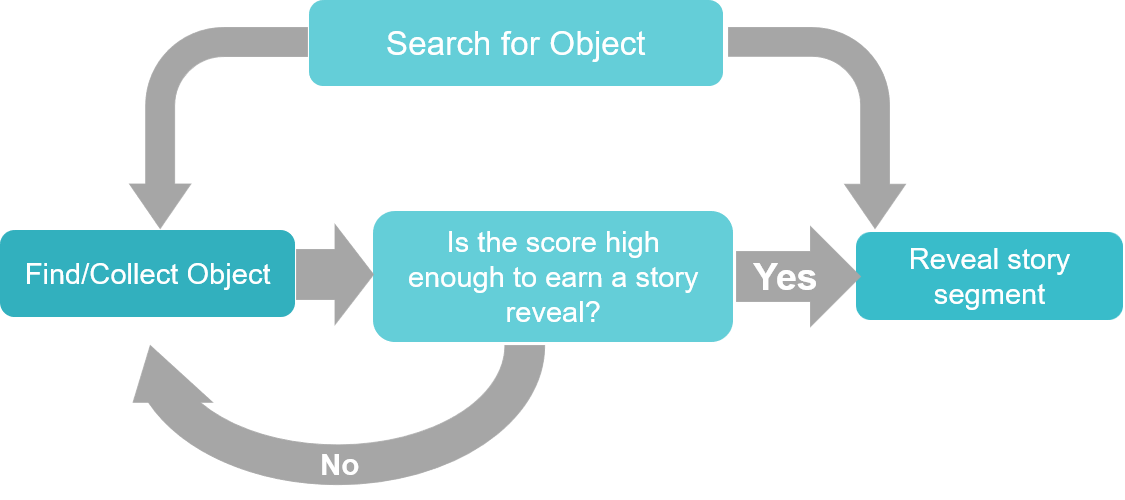
\includegraphics[width=2.5in]{imgs/Gameplay.png}
\caption{Description of the Gameplay}
\label{Gameplay}
\end{figure}

Given the rules, mechanics, and the location-based nature of the game, some data and database design considerations are:

\begin{enumerate}
	\item Nature of Geospatial Data. Learning data types, how they are stored, and how they may be obtained both from the player and by the player.
	\item Available DBMS. What databases and existing software packages work well with GPS data and are also capable of implementing game rules.
	\item Using Location Data. What computations can be done with GPS coordinates to enforce game rules and accomplish game mechanics such as the player interacting with geospatial objects.
	\item Database Schema. What entities and attributes are necessary to store and what portions of the game may be saved by the player.
\end{enumerate}
	
\section{High-level description of the system}
In order to be able to serve big number of requests in a timely manner and scale well with increasing number of players we need a system that will not only have a well designed, scalable database, but also other components integrated into a single, well thought architecture. Our system is built from 3 major components:

\begin{enumerate}
  \item Client-side application. We decided to support 2 major platforms that got widespread adoption: Android and iOS. For the proof-of-concept we focused on iOS. 
  \item Backend services, or middle layer. This component performs server-side operations, enforces gameplay rules and handles requests to our database. 
  \item Geospatially enabled database. Here all information regarding our players, objects and corresponding states is being kept. 
\end{enumerate}

We use following communication protocols between these components:

\begin{enumerate}[label=\Alph*]
\item REST over HTTP. This protocol is used to send messages from the client to the server sides and back
\item SQL. We use relational database and SQL over Application Layer to transform and query our data. 
\end{enumerate}

On the client side we use Apple’s Core Location Framework to collect longitude and latitude of a player and Apple’s ARKit to place objects around player. We calculate bearing and distance between player and a object to place objects around given user. To uniquely identify each player we use Vendor ID.
We want our backend to support large number of requests coming from multiple players. To achieve that we use multiple copies of the identical services capable to scale up or down depending on the level of load. Luckily we do not have to think about scalability properties of our hardware since we run our services in AWS Cloud on EC2 virtual instances.  To spread load across multiple copies of the backend service we use AWS load balancer that distributes client’s requests in a round-robin fashion between EC2 instances. 
We use AWS to host our database. 
Layout of all three components are represented schematically in \autoref{schema}. 

\begin{figure}
\centering
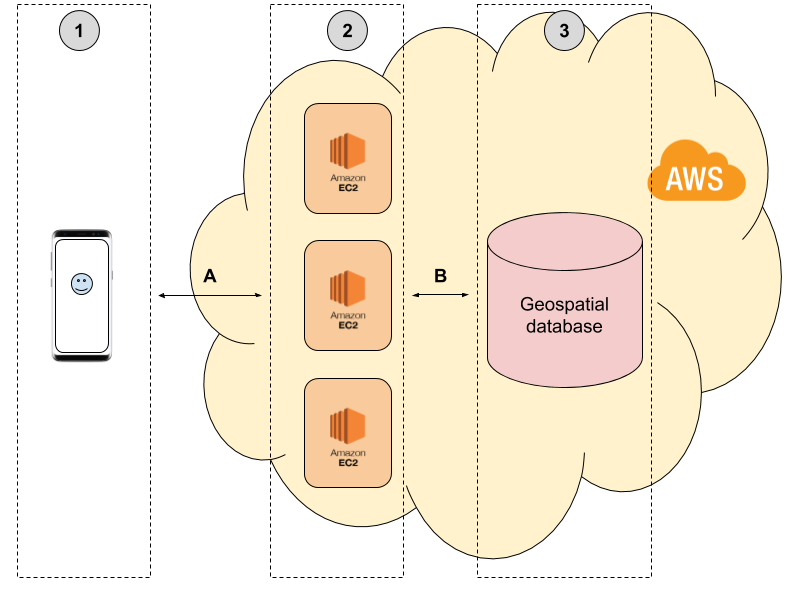
\includegraphics[width=2.5in]{imgs/systemschema.png}
\caption{Schematic layout of major components of the system}
\label{schema}
\end{figure}

\section{Database requirements and selection}

We defined the database requirements as follows:

\begin{itemize}

\item The database must be able to store the player’s information, including login ID, email, and country of location.
\item The database must be able to represent GPS location data. An important aspect when dealing with geospatial data is how to represent the data efficiently in order to reduce network traffic and storage requirements. A geospatial location is defined by its latitude and longitude coordinates. There are different formats in which these coordinates can be represented. The most common format for many applications (such as Google Maps and Geographical Information Systems or GIS) is the signed degrees format in which latitudes range from -90 to 90, and longitudes from -180 to 180.
\item The database can update the player's location. For the purpose of supporting the gameplay, it is important to update player’s locations when they move to a new destination where collectible objects are available. The database system must ensure the consistency and accuracy of the data even when the information of many closely-located players is been updated frequently. 
\item The location data must be stored with enough precision to support the actions of collecting objects. Latitude and longitude data are more precise when they use more decimals. Using 8 decimal places would give an exact location within 1 millimeter. We can achieve our desired precision using XX decimals. This information is important because it determines, along with the number of players, how much data is stored in the database. If the amount is very large, some sort of data compression would be necessary.
\item The system must have a function to calculate scores for each player, adding the value of the collected objects. The system also records subtotals for each object category and recognizes when thresholds are reached, triggering new story segments.
\item The database must be able to interface with the AWS platform where the data is stored, and the middle layer API.

\end{itemize}

We assessed four database options:

\begin{enumerate}

\item MySQL: This database provides support for spatial data formats, functions for the required calculations of scores, and a purpose-built MySQL database for integration with AWS. Another advantage is the simplicity of its interface and widespread usage due to its open source nature. Some disadvantages include: no support for dedicated calculations with geospatial data (distances, surfaces, etc.), and limited Scalability in case there are requirements to support a large number of players. 

\item PostgreSQL: PostGIS is a spatial database extention for PostgreSQL. It adds support for geographic objects allowing location queries to be run in SQL. The three features that PostGIS delivers to PostgreSQL DBMS are spatial types, indexes and functions such as distance, area, union, intersection, and specialty geometry. AWS offers a purpose-built PostGreSQL database. Another advantage is that PostgreSQL is the recommended relational database for working with Python applications, which are a essential component of the middle layer.

\item MongoDB: MongoDB is a document database with an expressive query language, support for secondary indexes and easy accommodation of changes in applications. The dynamic document data model of MongoDB removes the need for a central catalog describing the structure of documents. Every document is self-describing by defining the field names internally, which comes at the cost of greater use of space. Data is stored in the BSON format, a binary encoding of JSON, which does not compress data. 
Regarding location data, MongoDB offers geospatial indexes, which allows location data to be efficiently retrieved based on longitude and latitude. Such an index is useful only if records contain other fields beside location. It also offers support for AWS. The main disadvantage is that the support of more complex documents makes it less simple than a SQL database. 
 
\item Cassandra: Another popular NoSQL database is Cassandra. According to our research, however, the development of geospatial data indexing and retrieval features has been lacking for this database.  Recent research show how geohashing techniques can be used to index store data, converting the latitude/longitude information to a numeric geohash attribute and associating it to the data when being stored. However, this might make this database less attractive than the other options. 

\end{enumerate}

Based on this assessment, we selected the open-sourced PostgreSQL database, integrating the capabilities of the PostGIS extension. Apart from the aforementioned advantages of using these tools, our research indicates that PostGIS is close to becoming the standard to manage geolocation data for SQL databases.  This allows us to build a database with the following capabilities:

\begin{itemize}
\item	Once the data is uploaded, use simple SQL language to run complex queries related locations, objects, and other spatial data. 
\item Scale out the database in various ways: a. Manage a very large data size because it offers multi-TB capabilities, b. Handle a large amount of concurrency from the data, c. Use table-partitioning to break large data sets down into more manageable pieces.
\item Build custom functions using a language such as Python or R, which will be very useful to program the game requirements, rules and mechanisms into the database. 
\end{itemize}

\section{A Database design to support the gameplay}

The important entities that the database must be store are player data, object-category properties and locations, and story-segments, . As developers, we also need to know a player’s score in order to know what story segments the player has earned. Similarly, we need to know what objects have already been collected in order to not allow the player to collect them again. 

\begin{figure}[h]
\centering
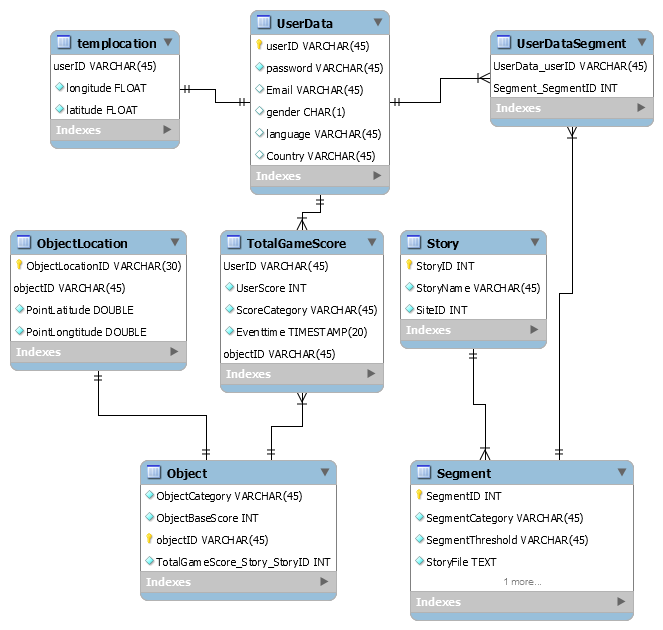
\includegraphics[width=2.8in]{imgs/DatabaseSchema.png}
\caption{Entity Relationship Diagram of Game Database}
\label{ERD}
\end{figure}

A list of geospatial points that correspond to viable latitudes and longitudes that can be used for any particular game will be stored separately from the list of geospatial points that are actually available to the player. This allows us to update the list and properties of physical geospatial points without affecting existing games and applications. A diagram of the database schema can be found above in \autoref{ERD}. 

\subsection{Players}
The UserData table contains login and personal information of all registered players taking part in the game. In the TempLocation table we store the player’s geographic location using the format provided by the PostGIS extension, which is a geographical object (latitude, longitude). We will collect the player's location using the API (see middle layer description). We will not store historical data of a player’s location, but simply update the current location.

 \subsection{Objects}
The Objects table includes a unique identifier (ObjectID), the object category (culture, economy or technology), and an attribute for the number of points awarded by each object (ObjectBAseScore). The game can run multiple stories, and therefore there’s a variety of objects that appear depending on the Story in which the player is immersed. This is why the StoryID attribute also appears on this table. 

The main mechanism of the game is collecting objects in different locations, which are described in the ObjectLocation table. The ObjectLocationID serves to record all the locations where objects can be collected. The latitude and longitude of the location are stored on this table, in order to match that information with the player’s location.

\subsection{Scores} 
The database needs to keep the player’s score and link it to the UserID, and this is done in the TotalGameScore table. The table records the score by object category and adds up the total UserScore. 

\subsection{Stories}
As players make progress through the game, collecting more objects and reaching predefined score thresholds, new segments of the story unfold until the player reaches the end. This information is stored in the Segment Table, which contains the SegmentID, the score Threshold that the user should achieve to unlock the segment, and a text StoryFile that is displayed on the device. 

The user will have several stories to choose from. These are stored in the Story table, which has a unique StoryID identifier along with the StoryName. 
Finally, in order to keep track of the User’s progress through the strory segments, by relating both entities in the UserDataSegment table. 

One major consideration in choice of database schema is to what extent the game may be housed on the player’s phone and what may be streamed from the central database. The former makes data integrity more feasible while the latter makes the storage of the player’s progress more feasible. For example, knowing what objects the player has already collected entails storing information that depends on both the player base and all of the objects’ geospatial locations. Hence, it merits its own table the size of the number of players times the number of object locations.  As the player base increases and the game is expanded, this table will grow very rapidly in size. However, if the player holds the object locations portion of the database on his or her phone, then the information may simply be stored as an indicator on the player’s downloaded schema. An example of the schema that can be saved on the player's phone lies below in\autoref{ERDUser}. 

\begin{figure}[H]
\centering
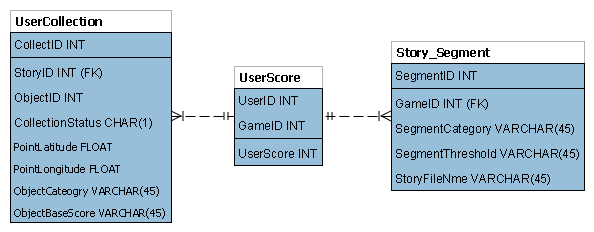
\includegraphics[width=2.7in]{imgs/MSDS7330_FinalProj_Prelim_ER2_USER.png}
\caption{ER Diagram of Database on User End}
\label{ERDUser}
\end{figure}

\section(Description of the middle layer API)

We use Python to create and RESTful API that connects the database with the ser interface. This middle layer performs the following operations:

\textbf{Player Registration:} Record user profile data (UserID, name, email address) from the client’s input on the mobile device. 
\textit{Details:}
@app.route('/api/game/user)
Input JSON format example: \big\{"userid" : "user01", "firstname" : "Arturo"\big\}


\textbf{Player State Synchronization:} Based on UserID, provide user data through a response to the client from the database.
\textit{Details:}
@app.route('/api/game/user/<userid>')
Input : UserID
Response JSON format : \big\{"userid" : "user01", "firstname" : "Arturo"\big\}

\textbf{Player location:} Instantaneously collect the player’s location data (latitude and longitude coordinates), and update this information in the database when the player moves according to the set thresholds (one update every XX).
\textit{Details:}
@app.route('/api/game/location‘)
Input JSON format example: \big\{"latitude":  "32.7877", "longitude" : " -96.8062"\big\}

\textbf{List of Objects around the player’s location:} Send a response to the client reporting all objects avaialbe for collection, based on current position within a specified radius.
\textit{Details:}
@app.route('/api/game/getlist/<userid>/<r>)
Input : UserID and Radius
Reponse JSON format : List of all available objects

\textbf{Colission report:} Send a response to the client reporting the game score and revealing new story segments, which are triggered according to the SegmentThreshold parameter in the database. 
\textit{Details:}
@app.route('/api/game/collection-reg‘)
Response JSON format : Current Score and Story Segment and story based on score

\textbf{User score status per Game category:} 
\textit{Details:}
API - @app.route('/api/game/user-score/<userid>‘)
Input : UserID
Response JSON format : ScoreCategory and Current score

\section{User and Server Interfaces}

Vlad: here are the ideas from the slide
We use Vendor ID to uniquely identify each player
We use Apple’s Core Location Framework to collect longitude and latitude of a player. We report his location approximately twice a second
We use Apple’s ARKit to place objects around player. To place objects all we need is to calculate bearing and distance between player and objects. 
We plan to share application via Apple’s TestFlight toolkit.
\begin{figure}
\centering
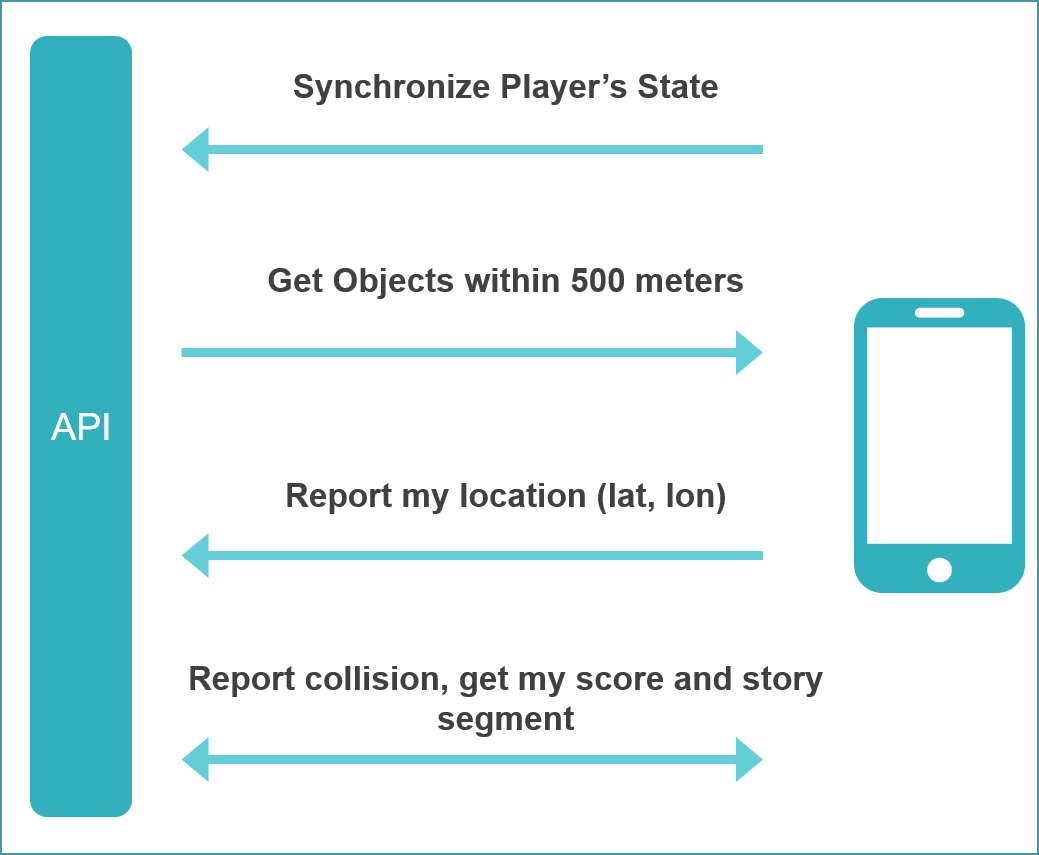
\includegraphics[width=2.5in]{imgs/UserInterface.png}
\caption{Diagram of User and Server Interfaces}
\label{UserInterface}
\end{figure}
Pictorial description above:

\section{Conclusion}

We developed a prototype of a geospatially-enabled game. We identified the following lessons and challenges:

\begin{enumerate}
\item Database and schema selection: there was no unique solution to meet the needs of our project. We found many options that offered different levels of performance, reliability, additional features.
\item Integration of APIs: We learned that the DBMS is just one element of the system. For the application to succeed we spent a large amount of time developing the middle layer.
\item Scalability: For the development of the prototype, the consideration of scalability was not very important. Our database selection would have changed if it was an immediate necessity. 
\end{enumerate}

\section*{Acknowledgment}


The authors would like to thank...


\begin{thebibliography}{1}
  
\bibitem{destination-engagement}
Koo Chulmo, Choi Kyuwon, Ham Juyeon, Chung Namho. Empirical Study About the PokémonGo Game and Destination Engagement, 2018

\bibitem{pokemon-motivation}
Marquet O, Alberico C, Adlakha D, Hipp JA. Examining motivations to play Pokemon Go and their influence on perceived
outcomes and physical activity. JMIR Serious Games 2017

\bibitem{location-based-mg}
L. Lehmann, Location-Based Mobile Games. GRIN Verlag Munich Germany, 2012.

\bibitem{data-store-issues}
J. Krumm and S. A. Shafer. Data store issues for location-based services. IEEE Data Eng. Bull., 2005.

\bibitem{location-based-services}
Jensen, C., Christensen, A., Pedersen, T., Pfoser, D.,Saltenis, S. and Tryfona, N. (2001). "Location-Based Services: A Database Perspective" Proceedings of Scandinavian GIS

\bibitem{massive-amounts-location-data}
K. Midtgård. Collecting massive amounts of location data in a NoSQL database. Master of Science in Computer Science, Norwegian University of Science and Technology, 2017

\bibitem{game-methodology}
R. Dillon, "The 6-11 Framework: A new methodology for game analysis and design" presented at the Proceedings Game-On Asia Conference, Singapore, Mar., 2011.

\bibitem{location-based-games}
L. Lehman, "Location-based Mobile Games" Technical University of Berlin, unpublished, 2012.

\bibitem {PostGIS scale}
Ramsey, Pau (2017)l. Scaling PostgreSQL and PostGIS, Dec 2017. URL: http://blog.cleverelephant.ca/2017/12/postgis-scaling.html

\end{thebibliography}

\end{document}


